\insertdesignoverview{Intake Mechanism}
{Drive into the crater and intake silver minerals; sort out the gold minerals} % Goals of the mechanism
{intake_CAD.PNG}% CAD Image
{intake_build.JPG}% Build Image
{0.25" Medium Density Fiberboard, Rubber Bands, VEX chain, Aluminum, ABS Plastic, Carbon Fiber, Skewers}% Materials ex. 0.25" MDF, Aluminum, etc
{Laser Cutting, 3D Printing}% Manufacturing Processes ex. Laser Cut, 3D print, etc.
\subsection*{How it Works}
Our intake mechanism features laser cut sprockers with rubber bands in between the teeth. The intake spins due to a chain and sprocket powered by a VEX motor. The minerals are fed into the intake and roll up strategically placed dowels to sort the minerals. The gold mineral, being smaller in size, goes through the intake and falls out the back of the dowels. The silver mineral, being larger, gets stuck in the intake and waits for the transfer mechanism. Refer to Figure \ref{fig:sorting} for an image of this passive sorter. 

\begin{figure}[h!]
\centering
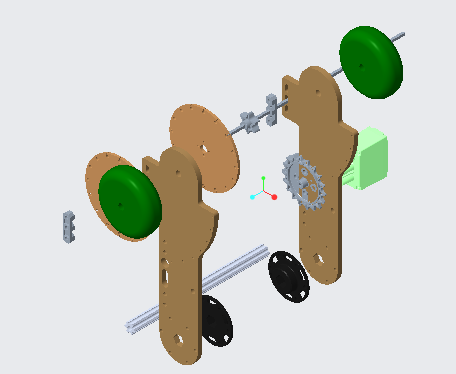
\includegraphics[width=0.8\textwidth]{Design_Overview/exploded_intake.PNG}
\caption{Exploded View of the Intake Mechanism}
\label{fig:exploded_intake}
\end{figure}

\begin{figure}[h!]
\centering
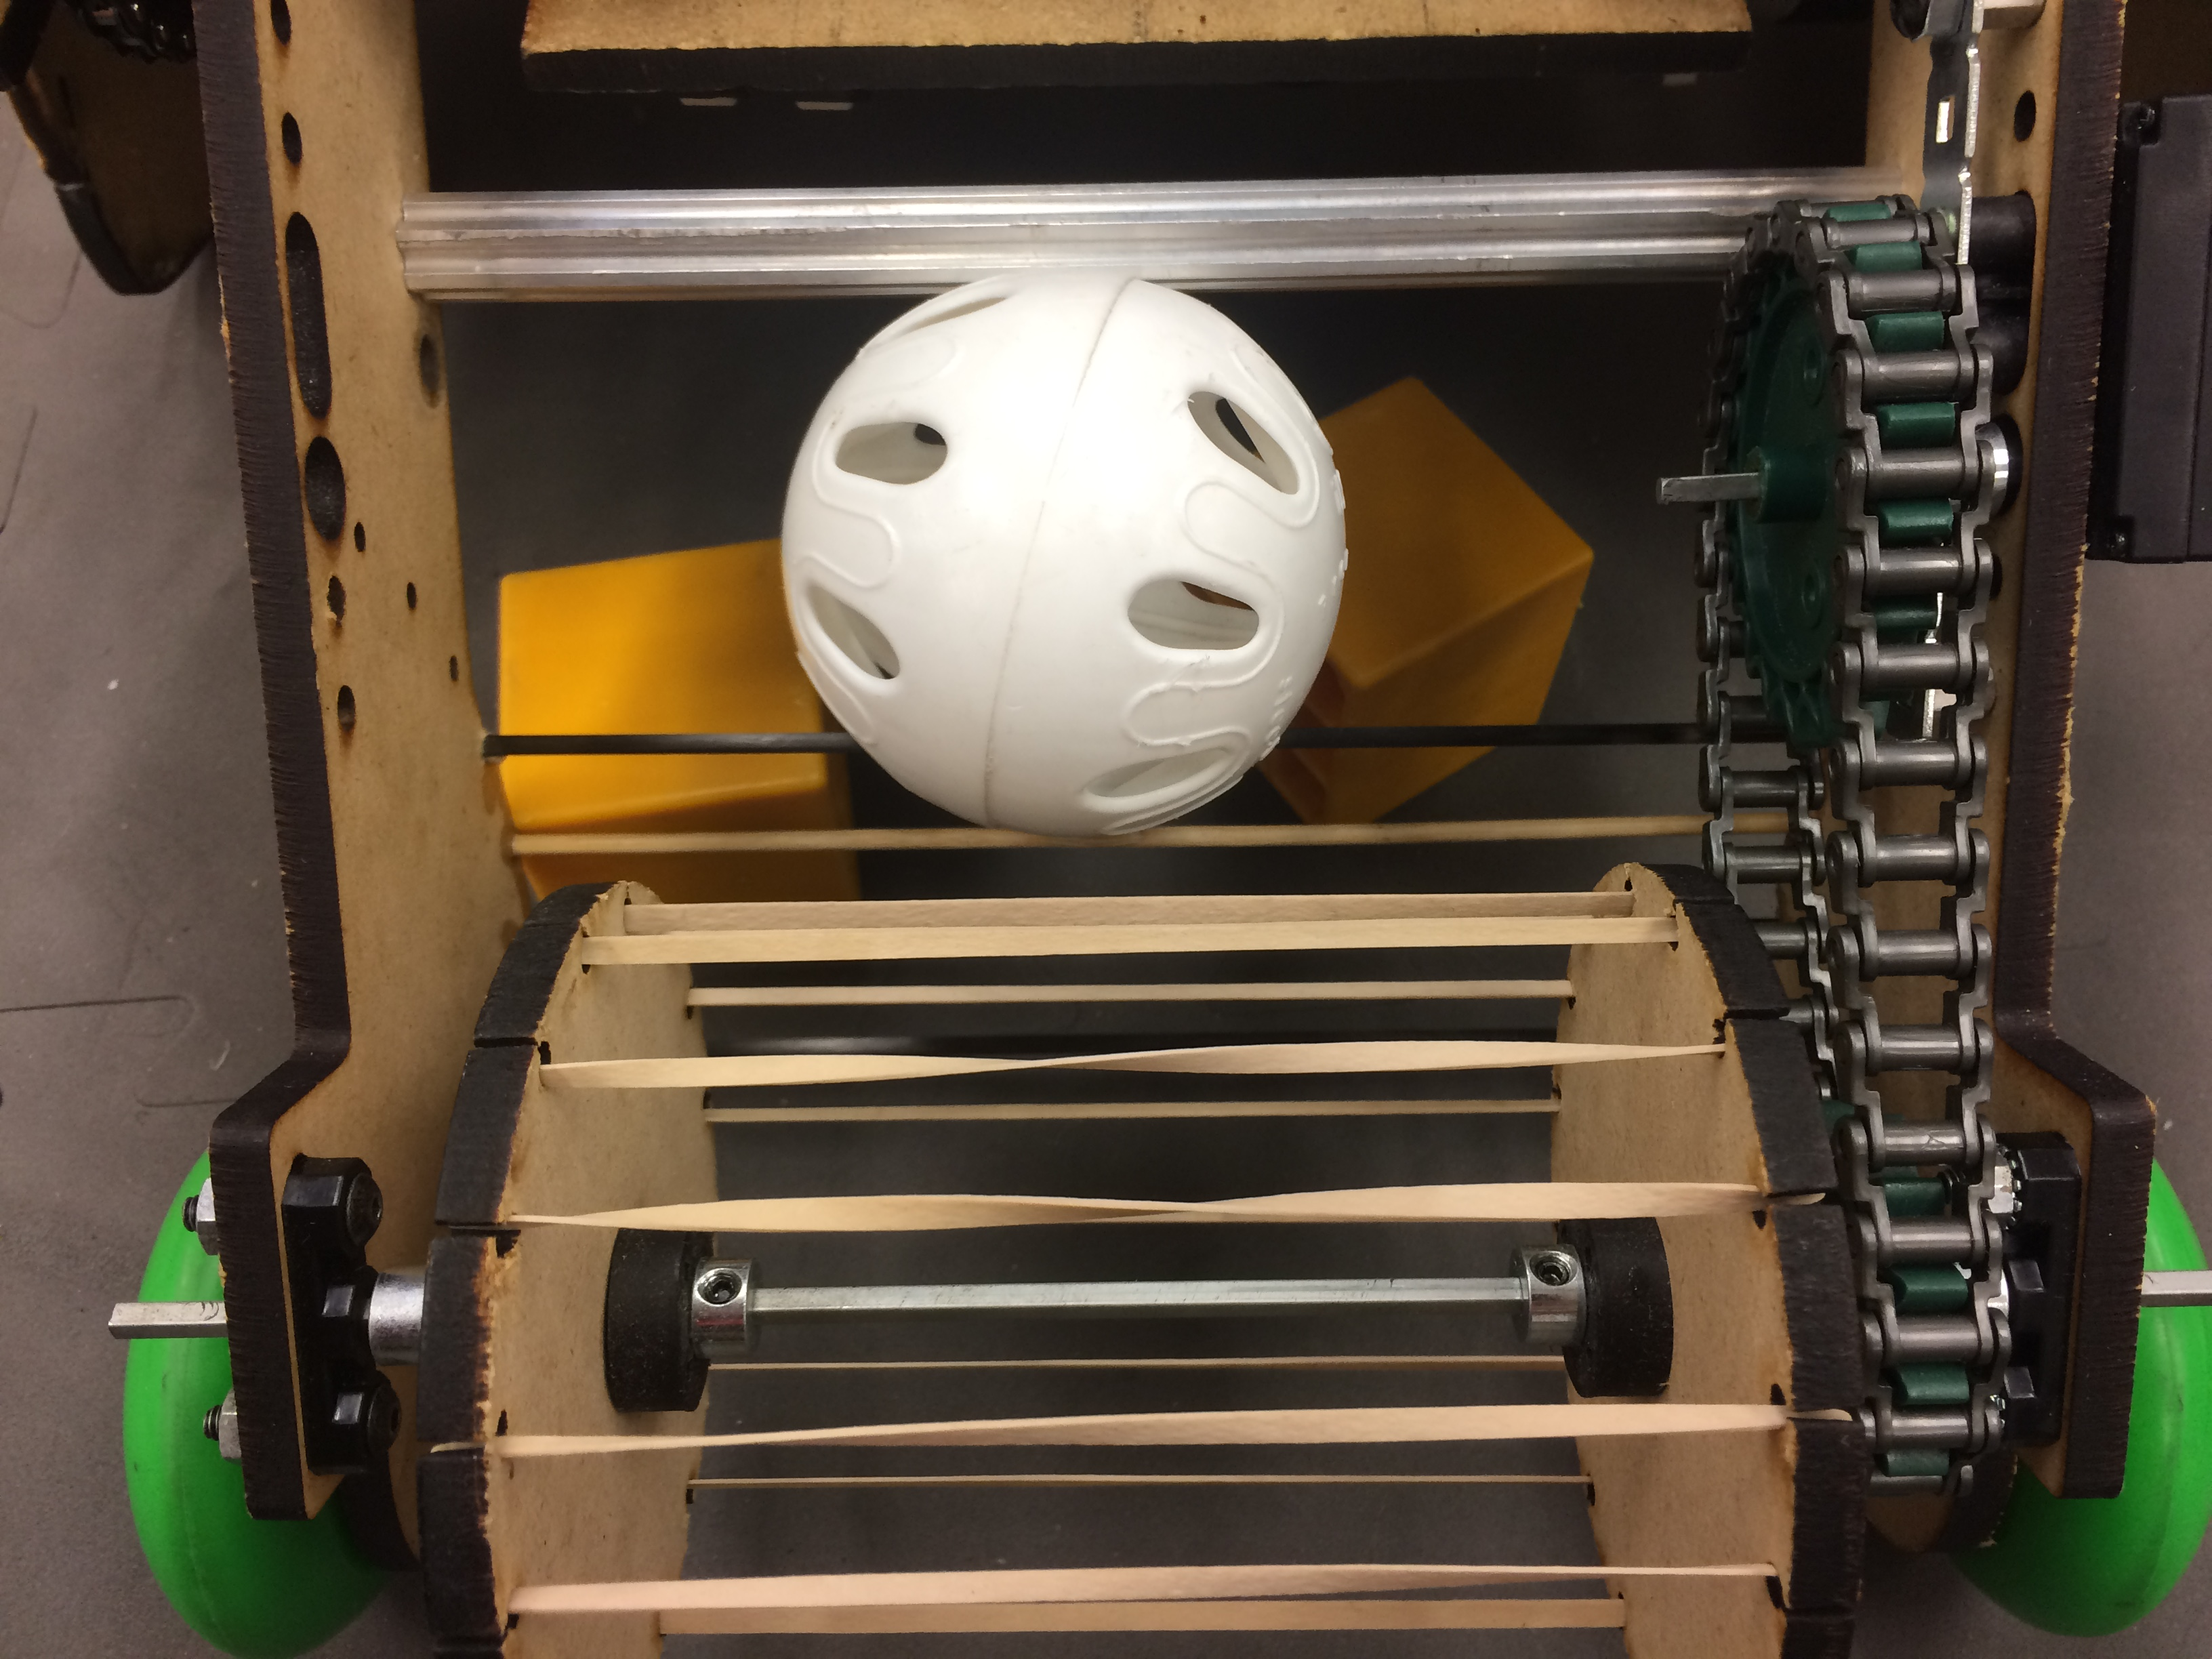
\includegraphics[width=0.8\textwidth]{Design_Overview/Sorting.JPG}
\caption{Passive Sorting}
\label{fig:sorting}
\end{figure}

\subsection*{Modelling \& Simulation}
Much like all of our other mechanisms, we designed and simulated the intake using body and motion skeletons in PTC Creo. The most challenging issue with designing the intake was determining how far forward the rubberband wheels would be, as well as the size of the wheel itself. To make this easier on ourselves, we created sketches of the silver and gold minerals in the body skeleton and referenced it to design a smooth curve upwards that would maintain contact with the intake wheel. \hl{Our use of skeletons makes part implementation simple and fast, and facilitated continuous design iteration.} See below in Figures \ref{fig:skel_intake} and \ref{fig:skel_intake_use} to see how we implemented skeletons into our design. 

   \begin{figure}[ht!]
	\centering
	\begin{minipage}{.48\textwidth}
	  \centering
	  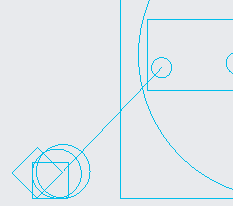
\includegraphics[width=0.8\linewidth]{Design_Overview/skel_intake.PNG}
	  \caption{The Intake Arm and Minerals in the Body Skeleton}
	  \label{fig:skel_intake}
	\end{minipage}%
	\begin{minipage}{.48\textwidth}
	  \centering
	  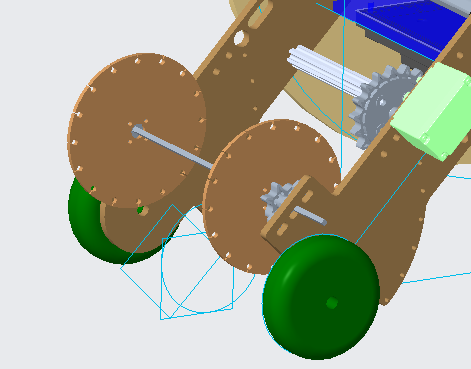
\includegraphics[width=0.8\linewidth]{Design_Overview/skel_intake_in_use.PNG}
	  \caption{The Skeleton in Use with Intake}
	  \label{fig:skel_intake_use}
	\end{minipage}
	\end{figure}

\subsection*{The Phillip Mech}
At the back of the intake, we have a mechanism to transfer the silver into the shooter (something our team refers to as Phillip). This consits of a REV servo that flips up. The arm is made of laser cut mdf made to have specially bent piano wire that works by having the intake bend the piano wire slightly out to get the silver in and then bends back to normal when the silver gets all the way in. The reason we use piano wire is that it holds its shape really well which means that it is hard to bend permanently but is easy to flex outward to allow for the silver to fall into the tray that goes up to the shooter.

   \begin{figure}[ht!]
	\centering
	\begin{minipage}{.48\textwidth}
	  \centering
	  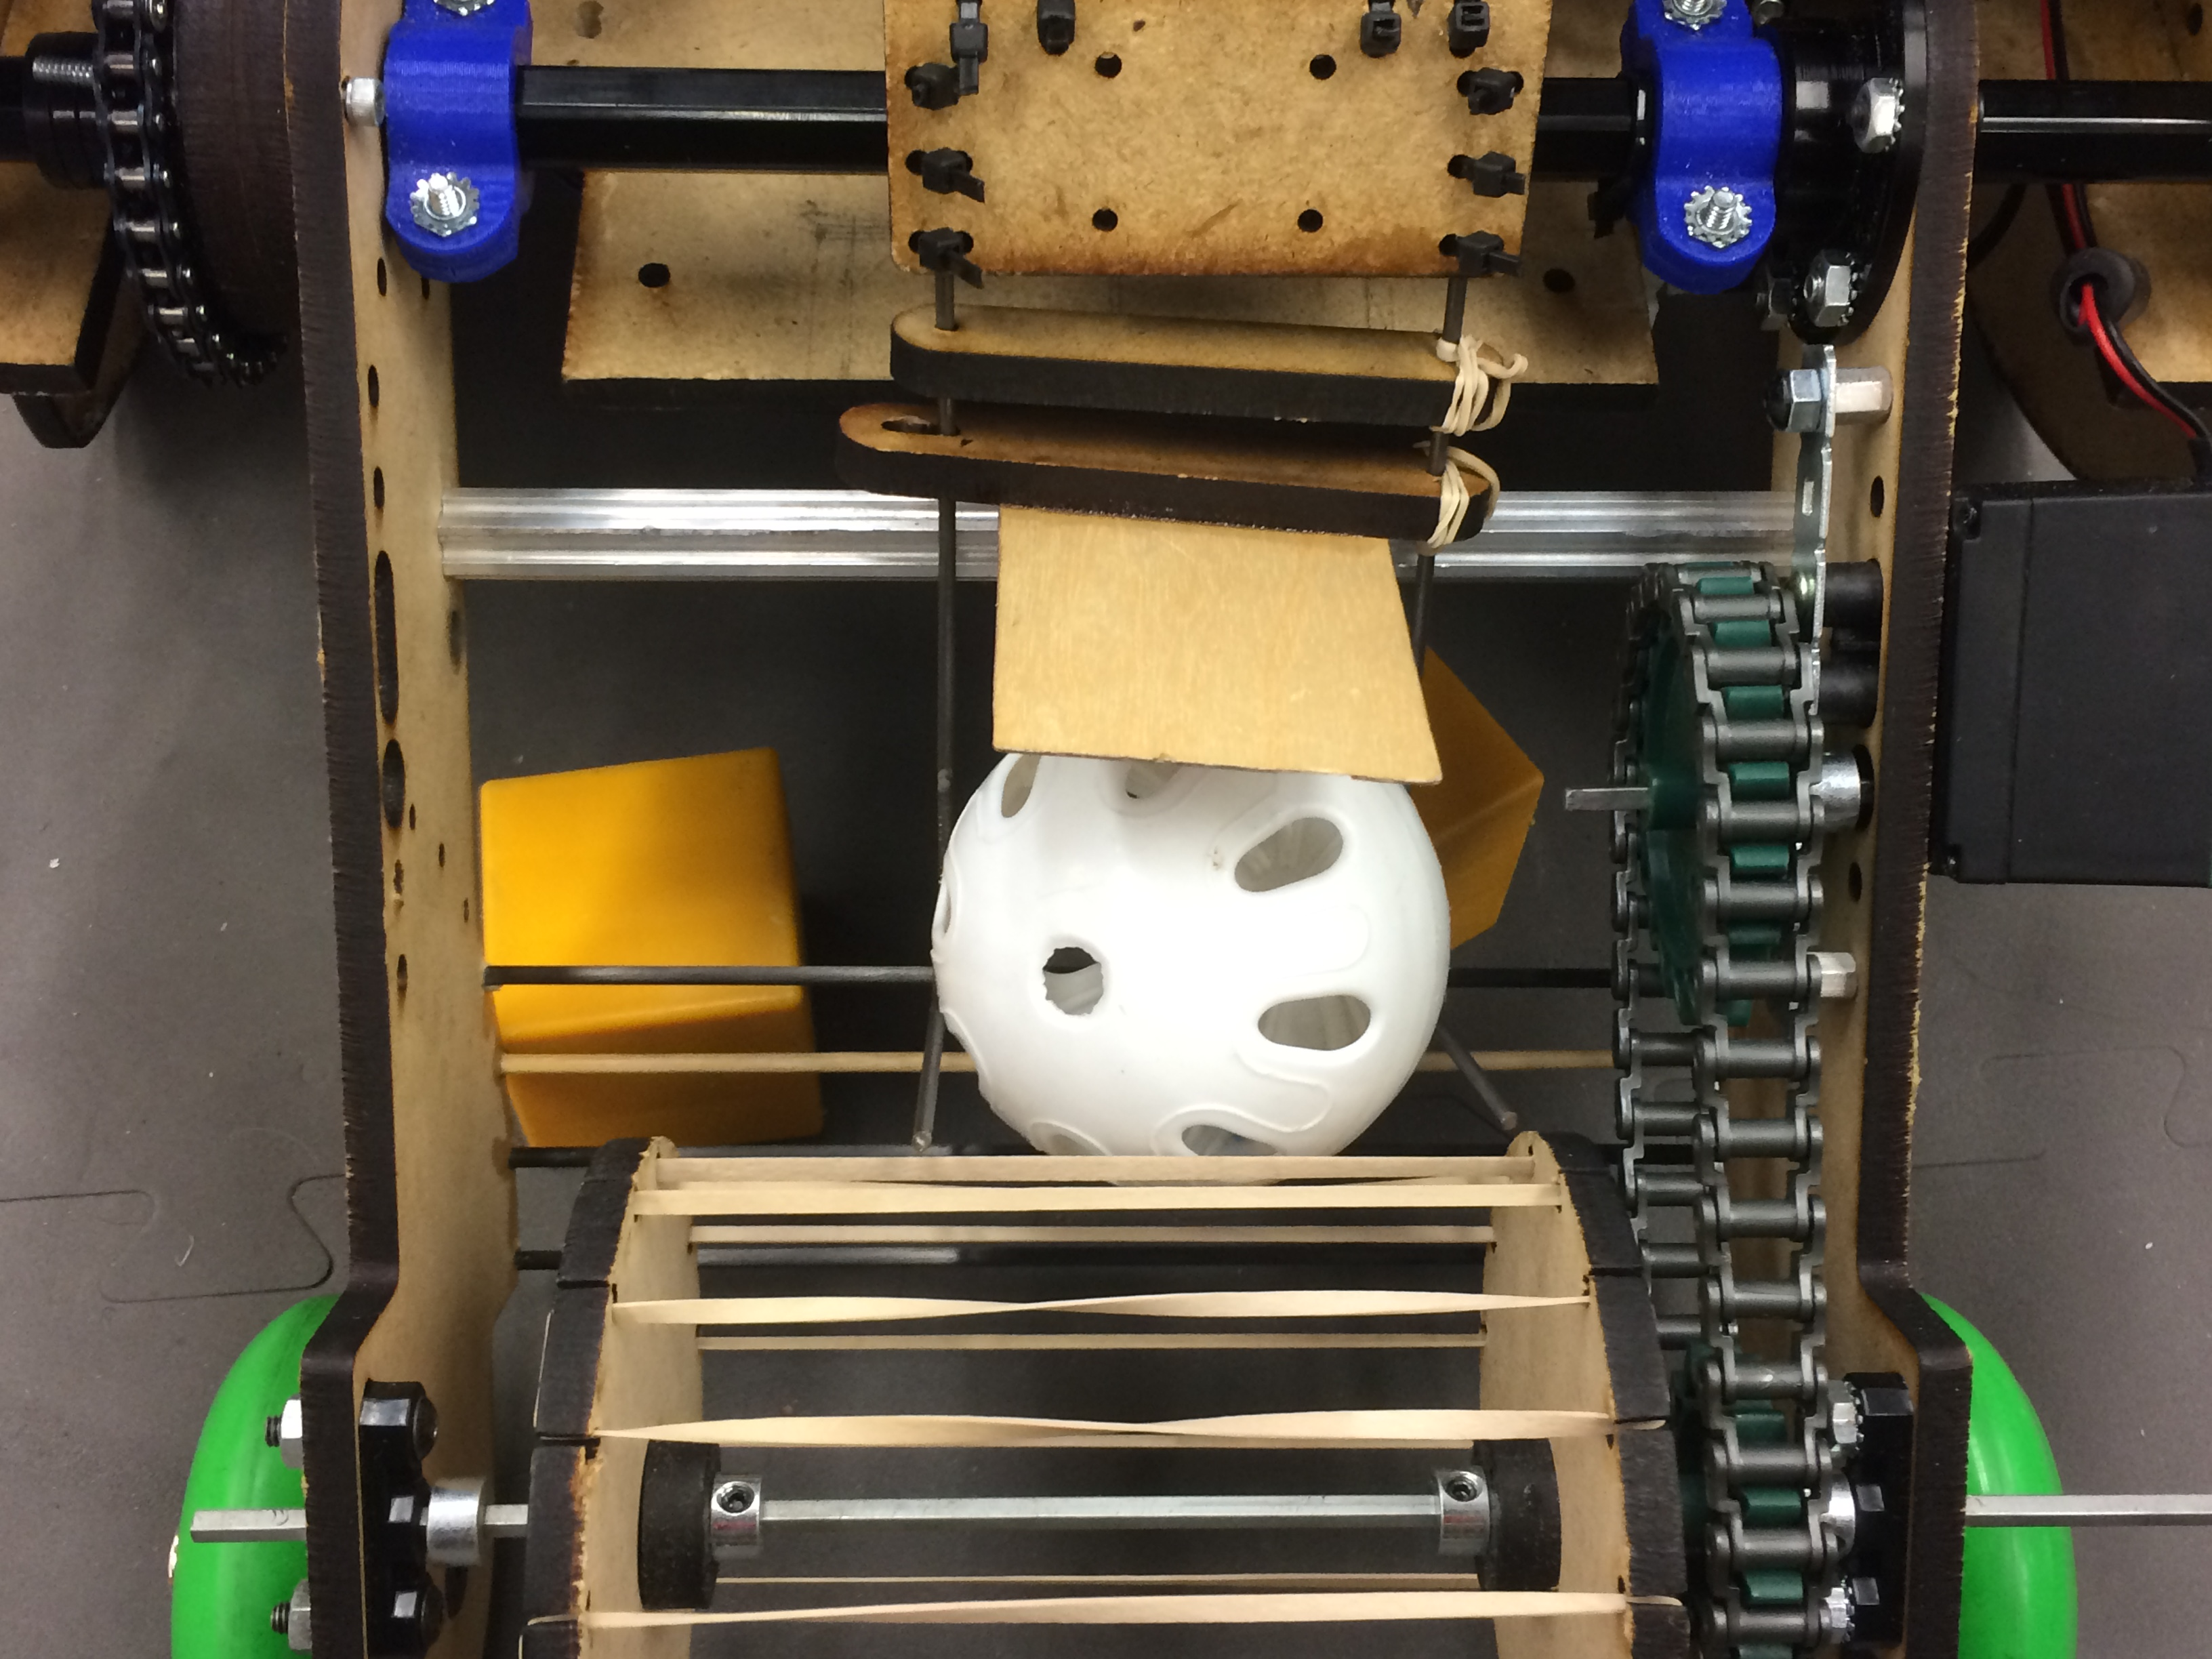
\includegraphics[width=0.8\linewidth]{Design_Overview/Phillip_1.JPG}
	  \caption{Loading The Transfer Mechanism}
	\end{minipage}%
	\begin{minipage}{.48\textwidth}
	  \centering
	  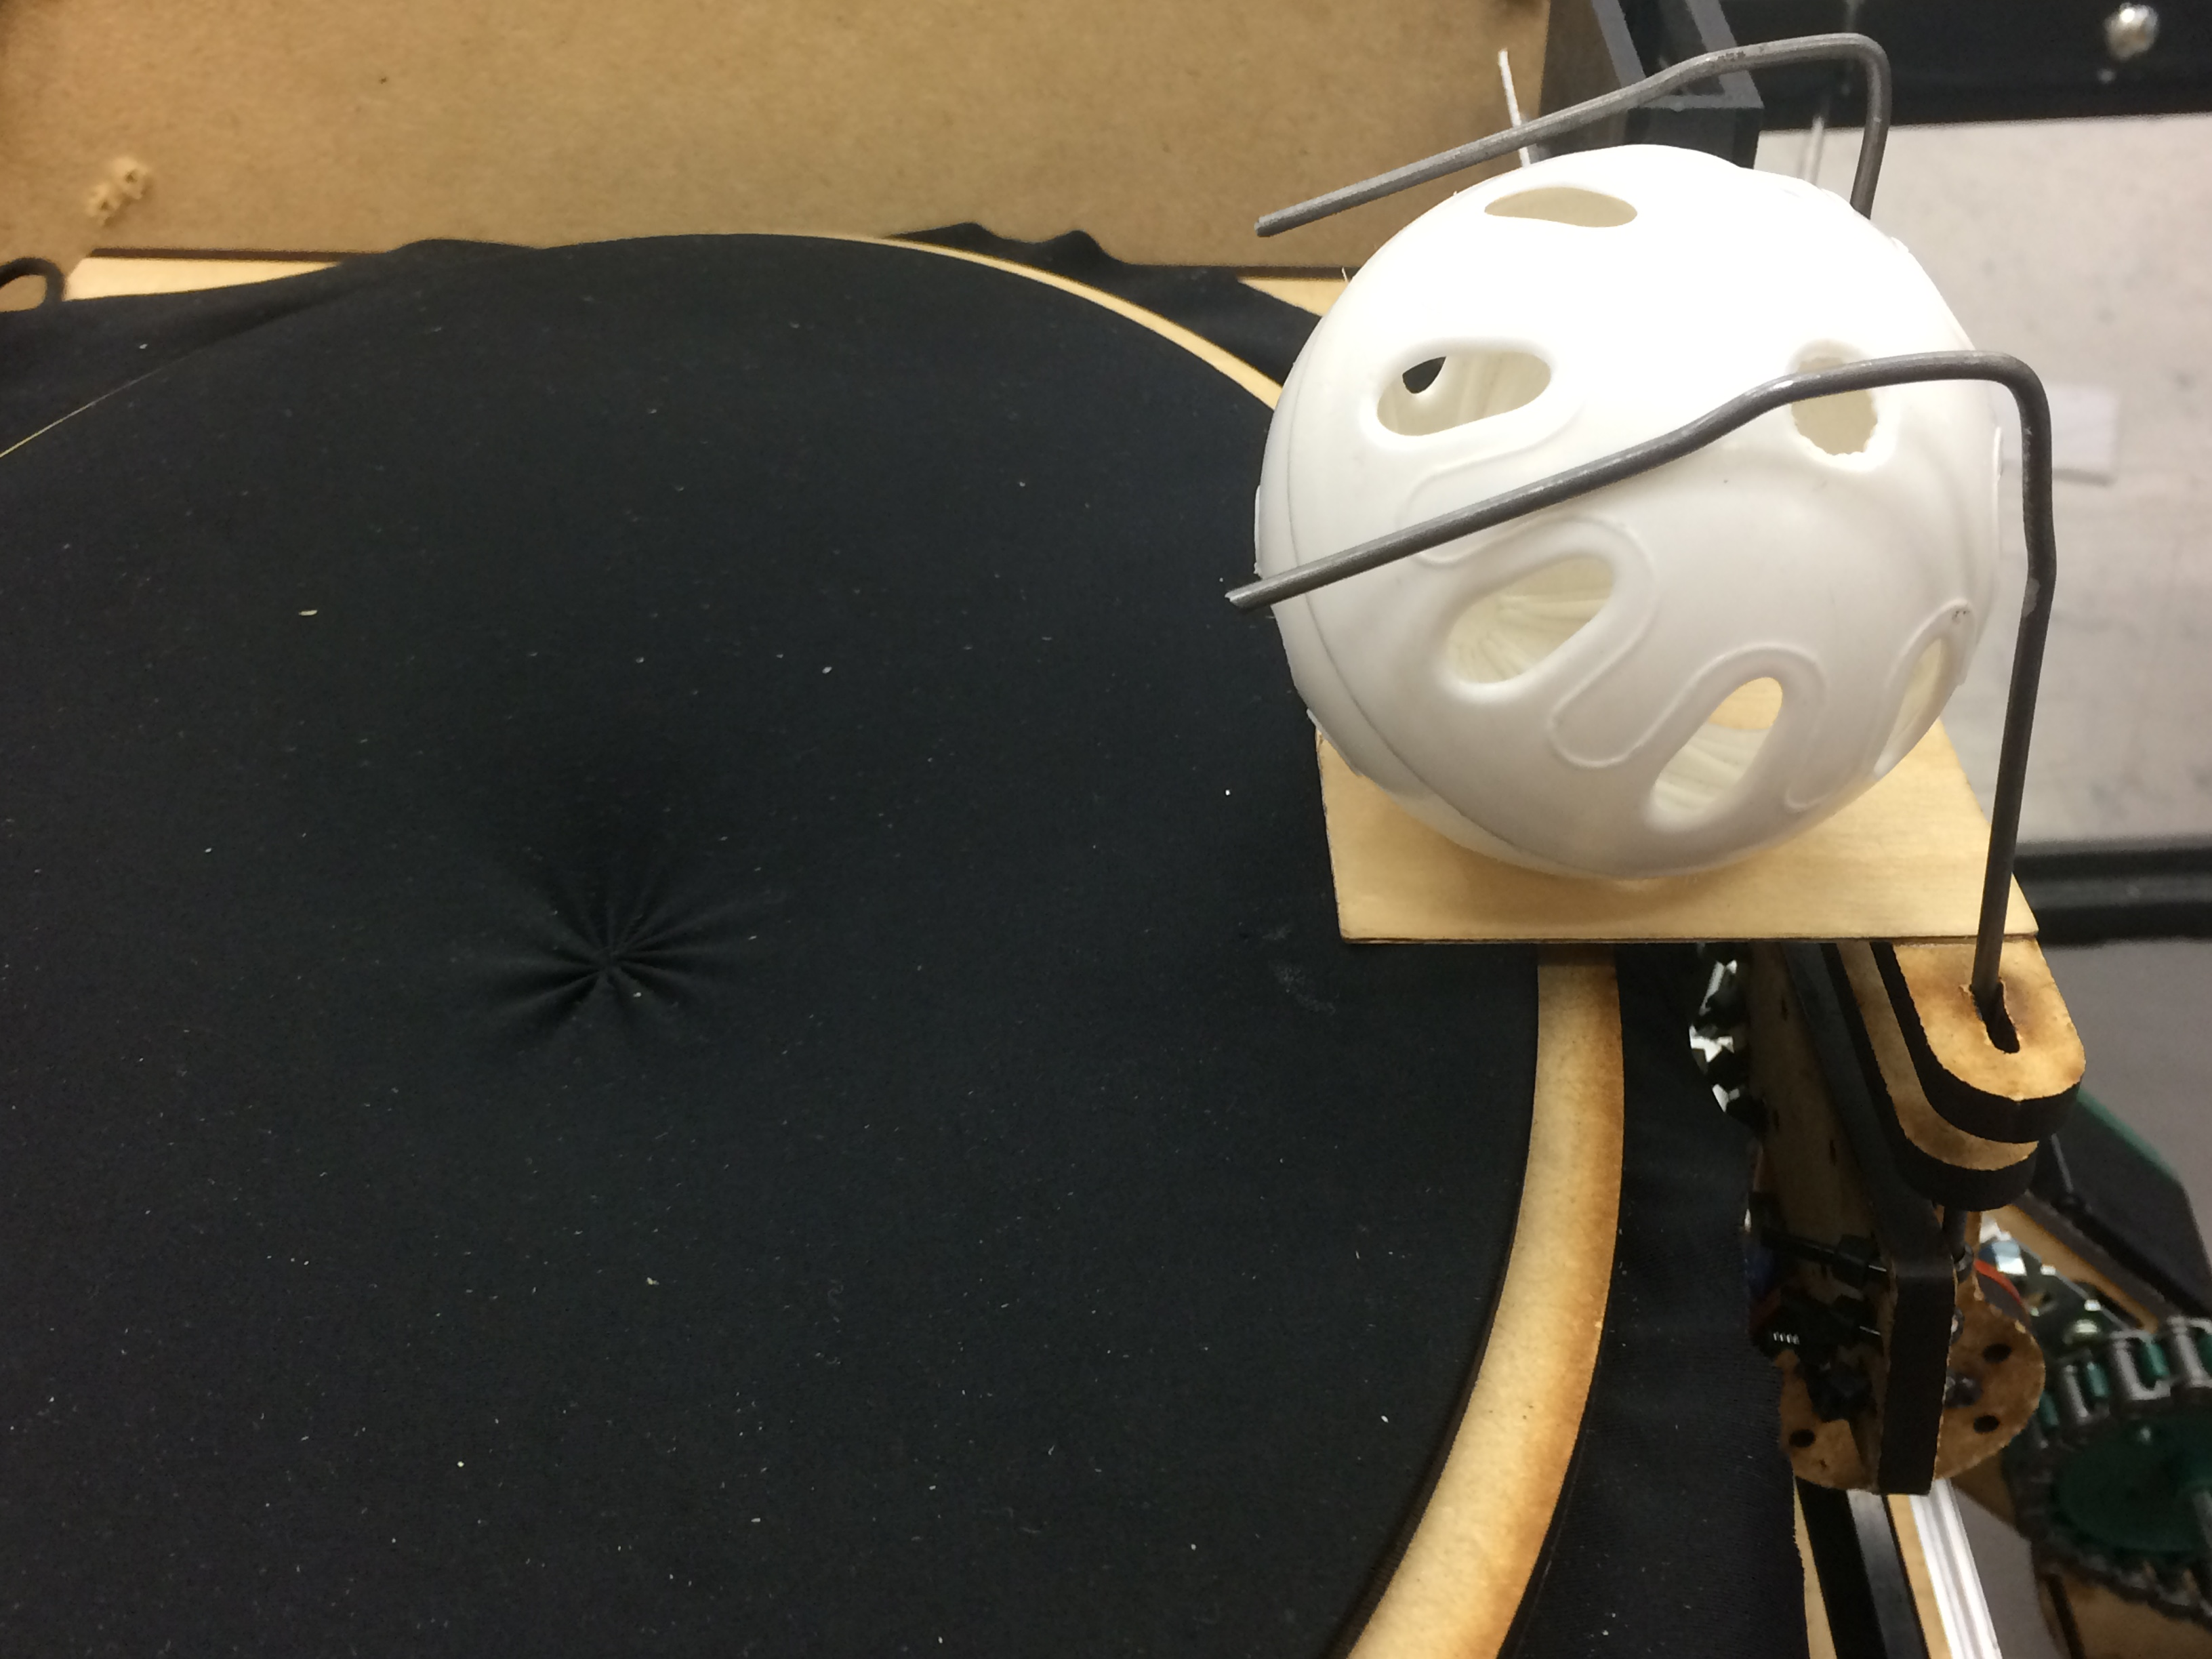
\includegraphics[width=0.8\linewidth]{Design_Overview/Phillip_2.JPG}
	  \caption{Transfer Mechanism Deposit to the Shooter}
	\end{minipage}
	\end{figure}

\subsection*{Iterations}
The placement and size of the rubber band wheels took several iterations to complete. We struggled with figuring out where we'd need to place it in order to pull in minerals smoothly, and used the robot's body skeleton as well as several stages of prototyping to figure it out. In addition, we changed our geared intake to one with a chain and sprocket in order to move it further back up onto the arm. After our first prototype, we also replaced an intake plate with strategically placed dowels for sorting. 

\interesting{Iterative Design with the Intake}{design:6}

\begin{figure}[htp]
\centering
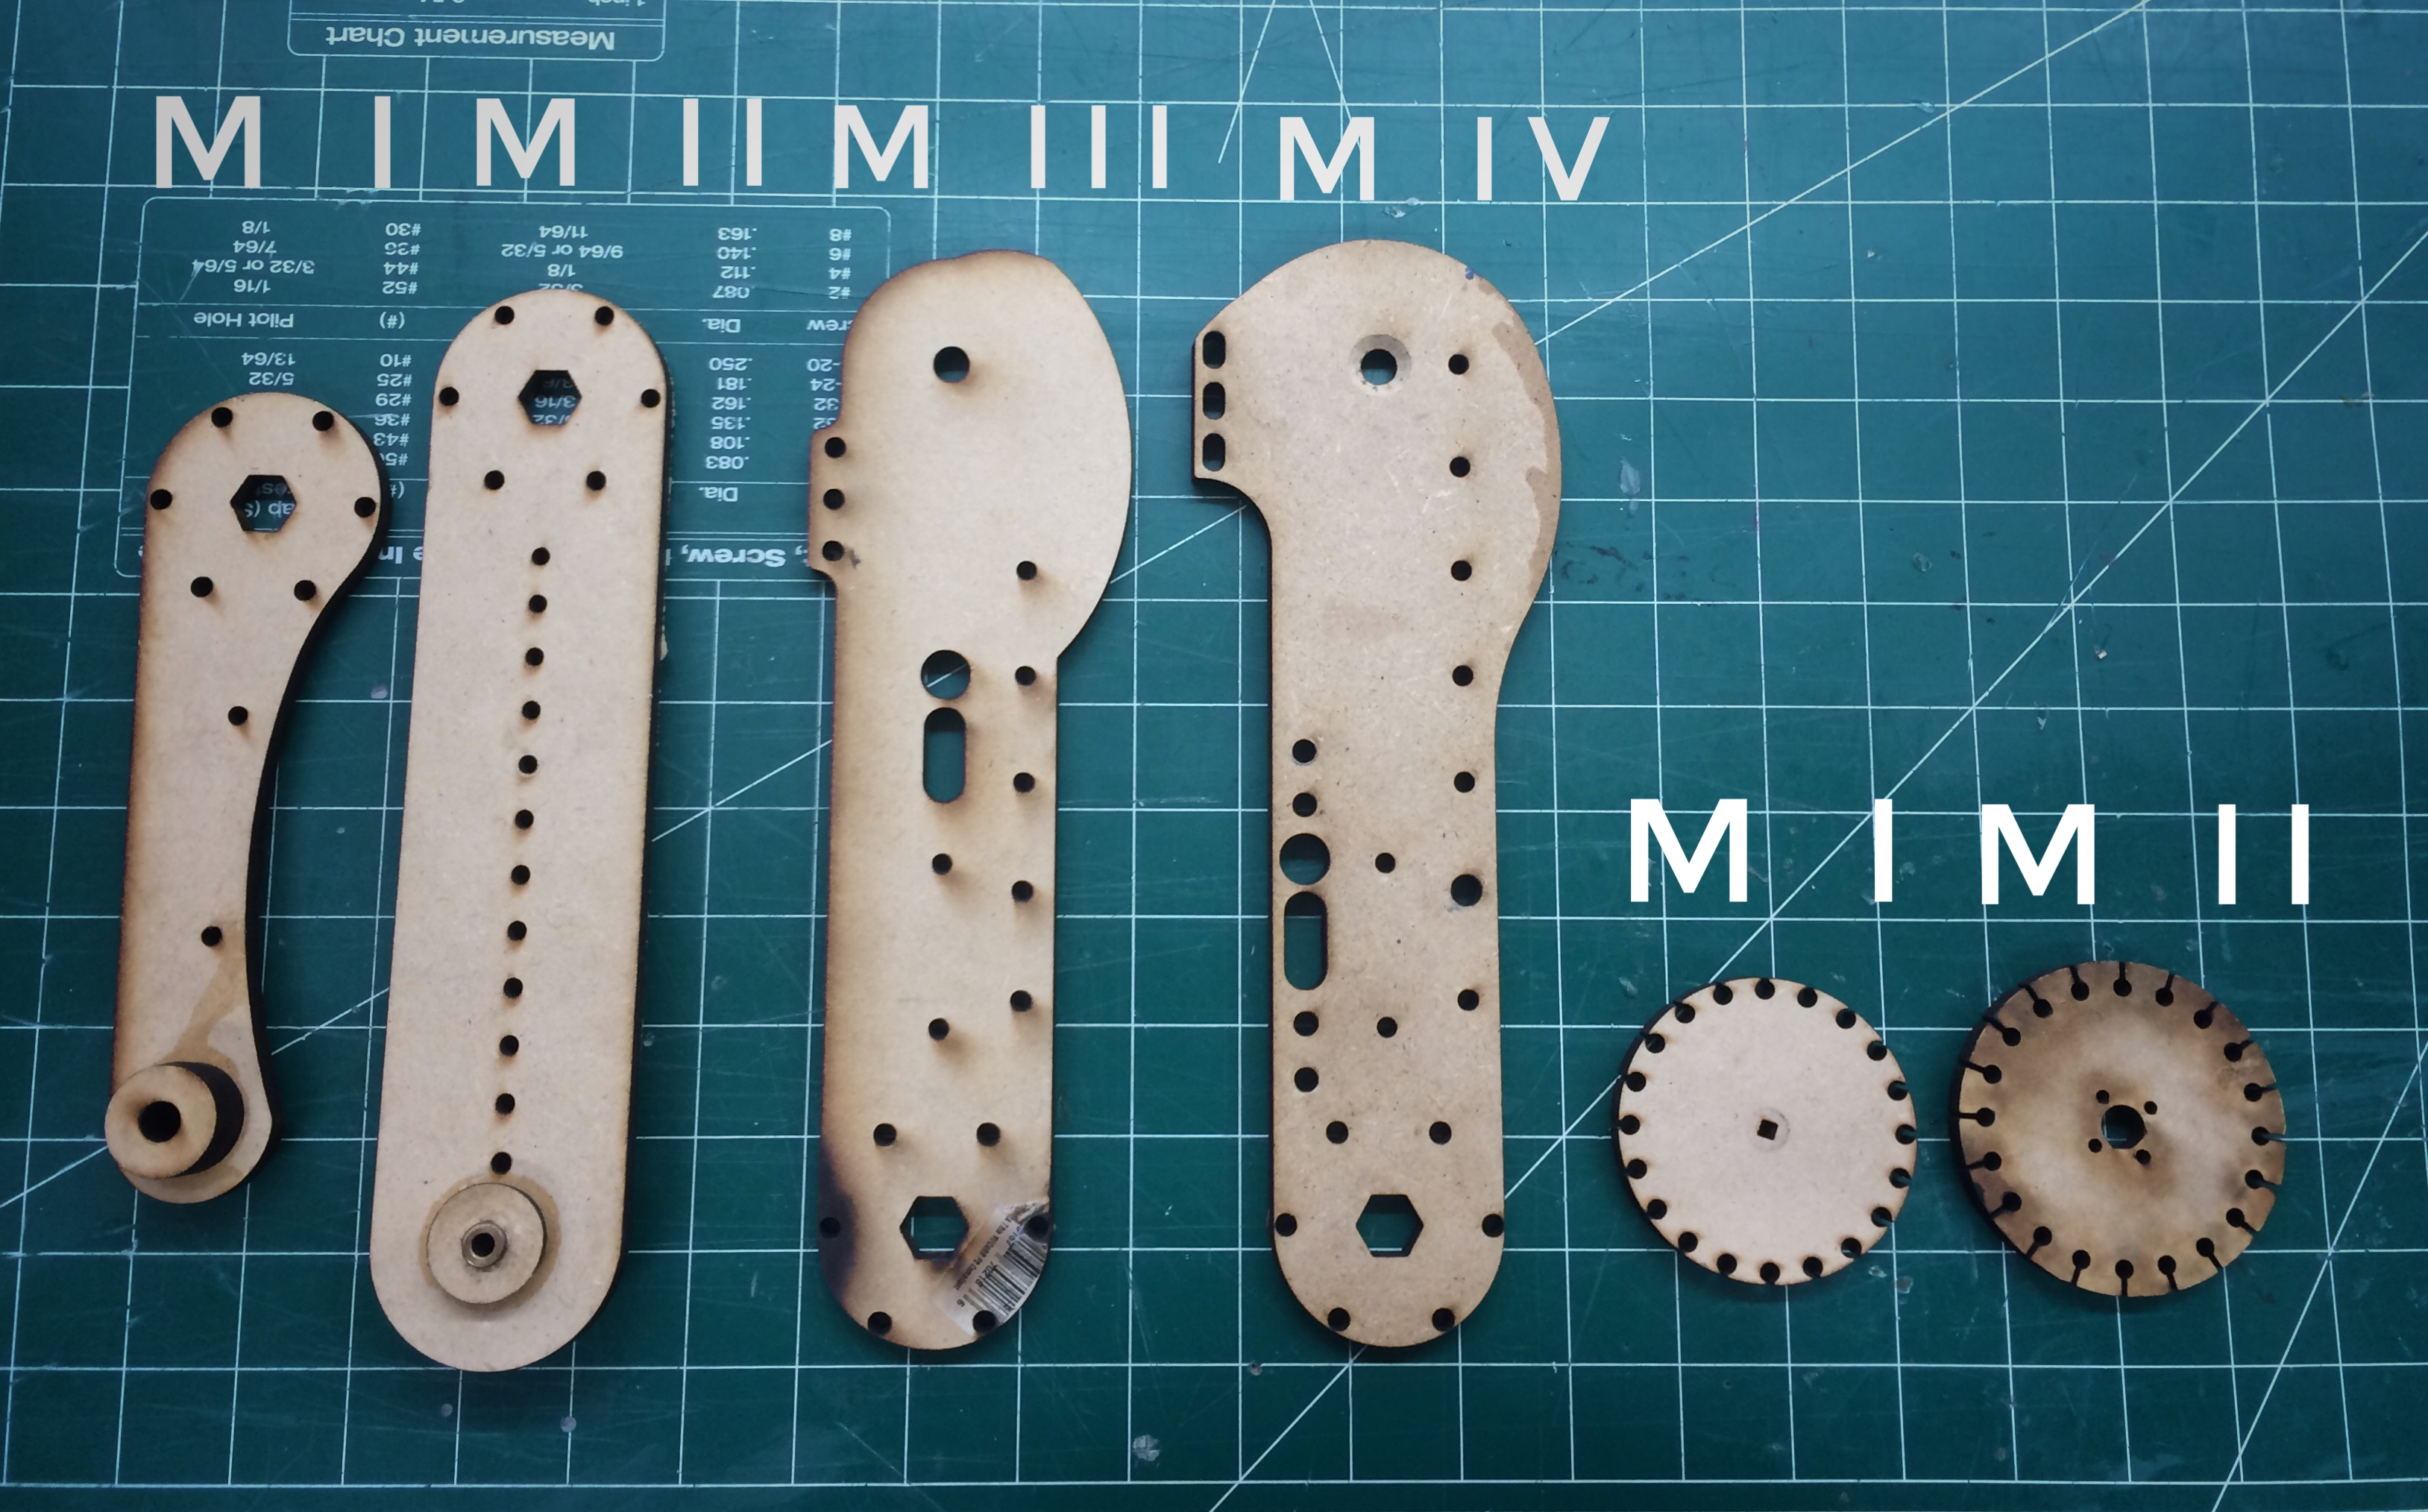
\includegraphics[width=.8\linewidth]{Design_Overview/Intake_Iteration.jpg}
\caption{Design Iteration of the Intake, Mark I to IV}
\label{fig:intake_it}
\end{figure}

\begin{figure}[htp]
\centering
\begin{minipage}{.32\textwidth}
  \centering
  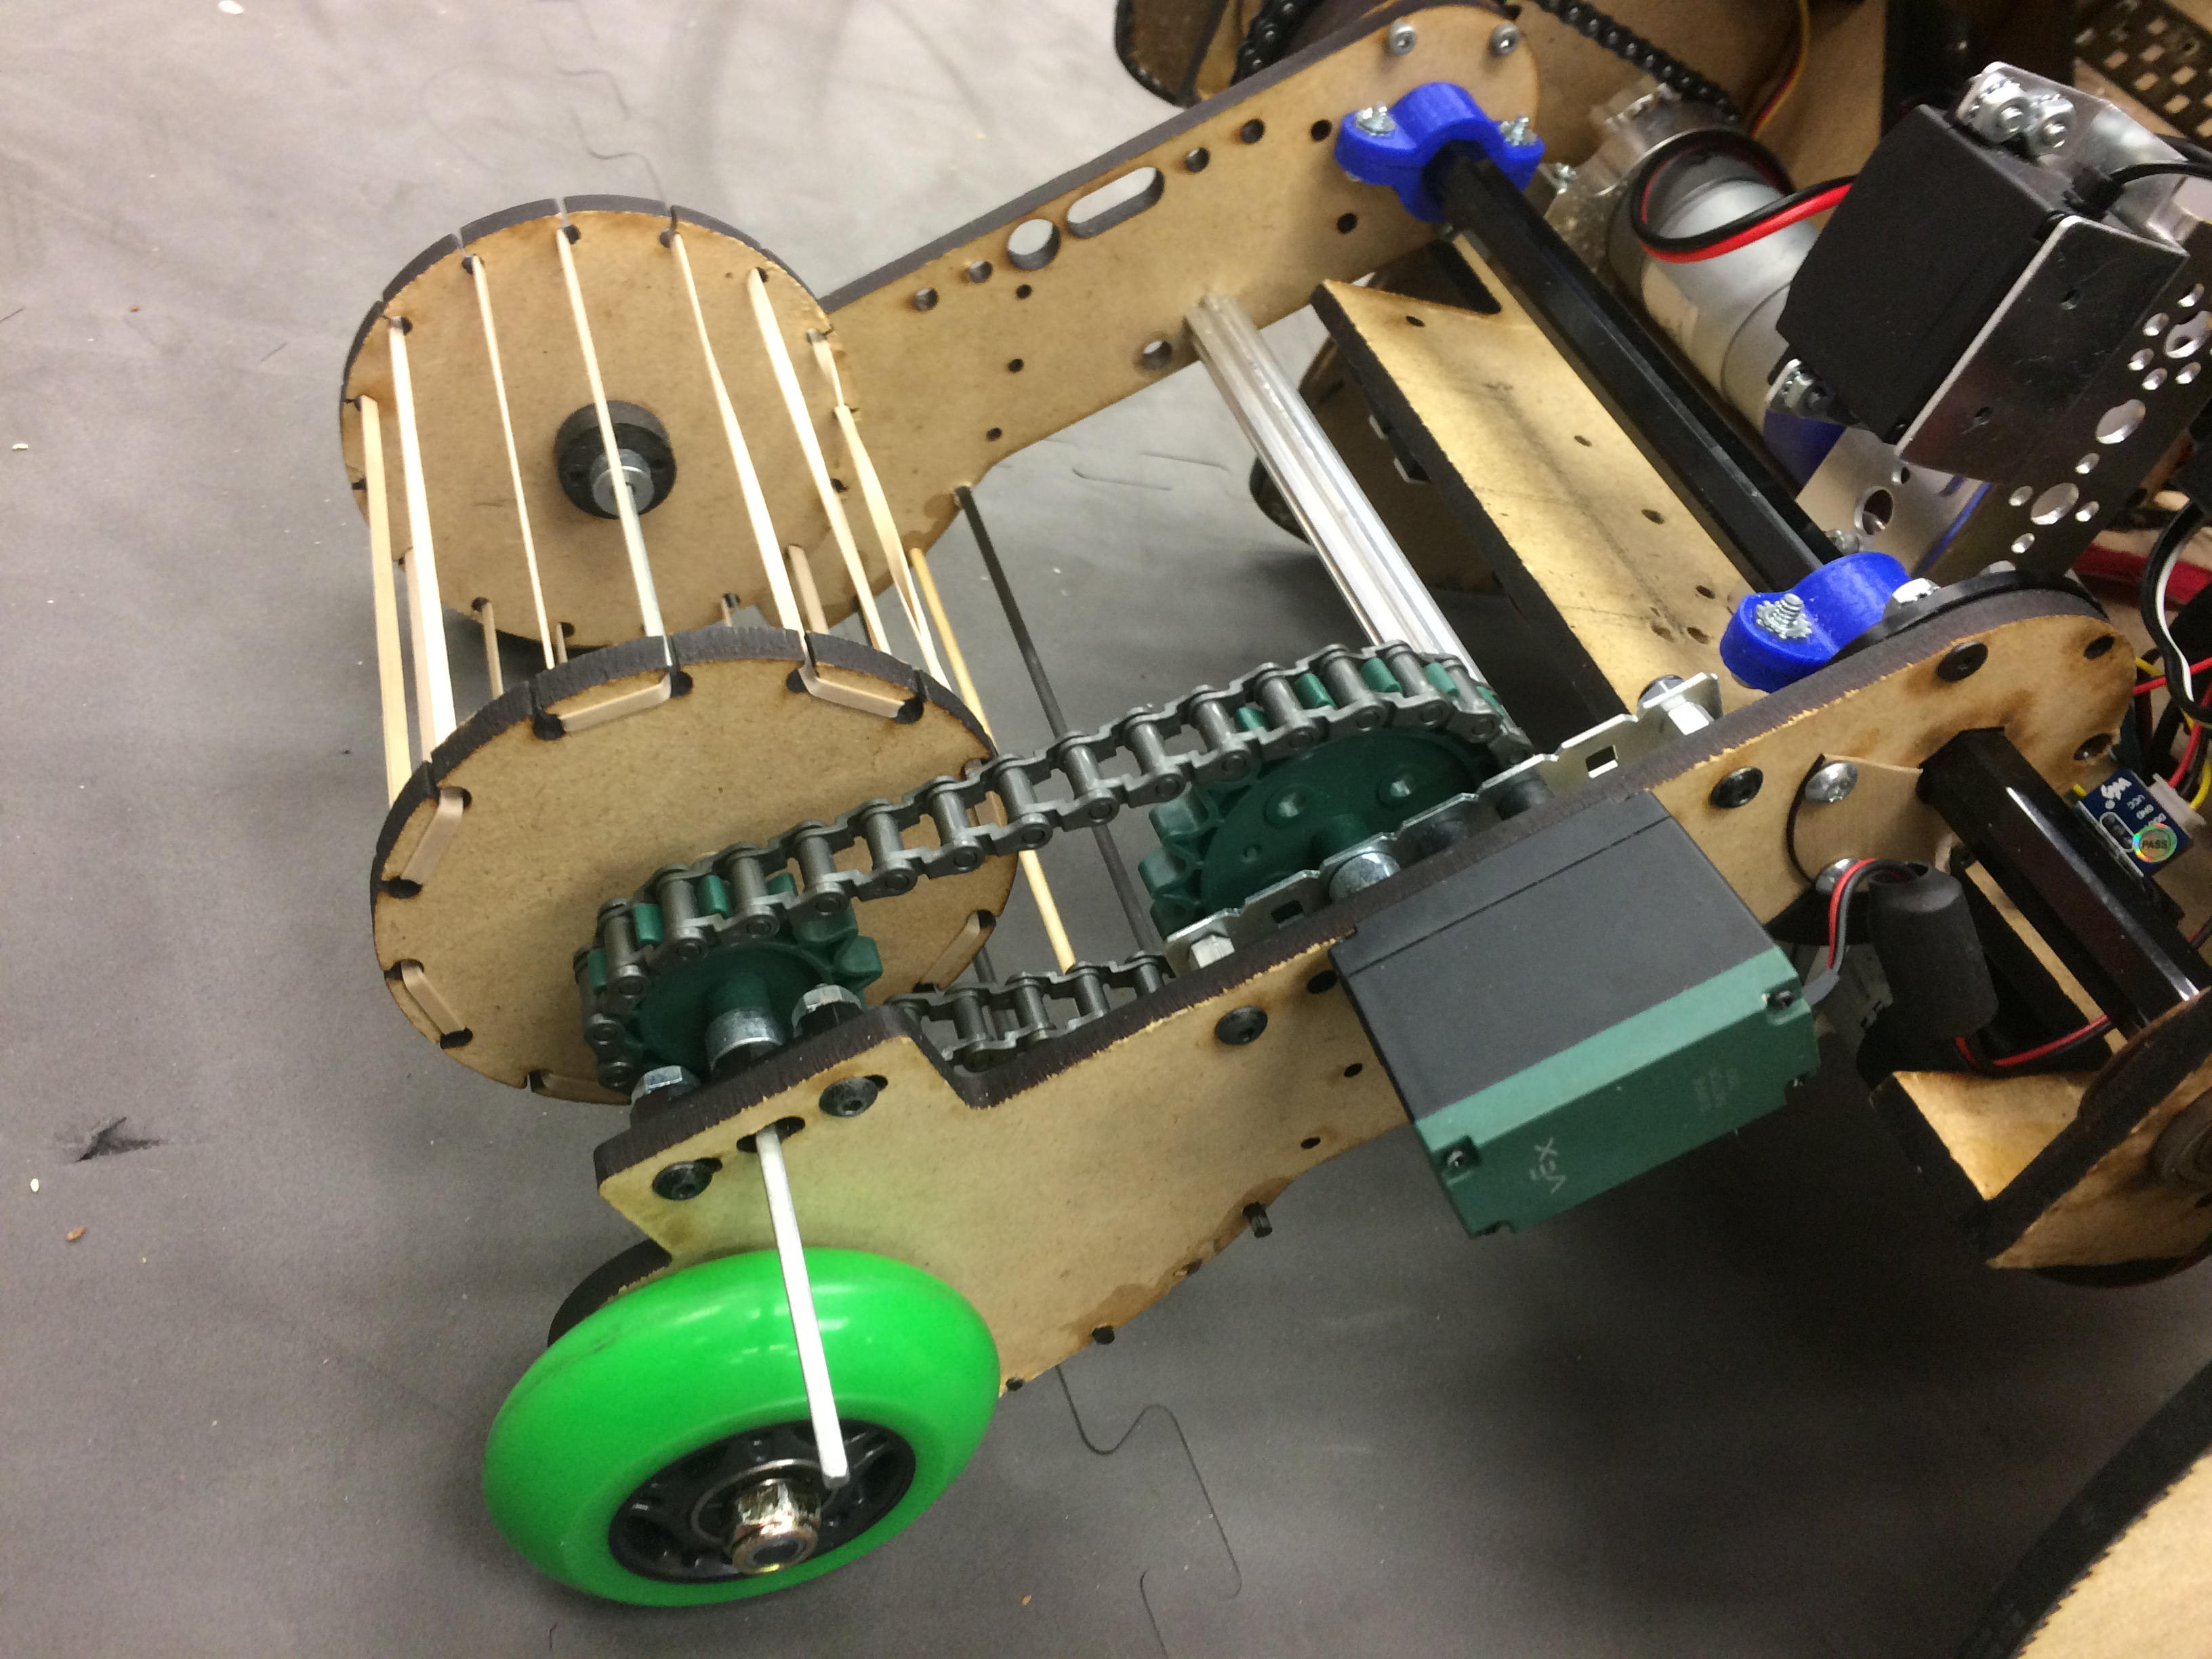
\includegraphics[width= .9\linewidth]{Design_Overview/Intake_Left.JPG}
\end{minipage}%
\hfill
\begin{minipage}{.32\textwidth}
  \centering
  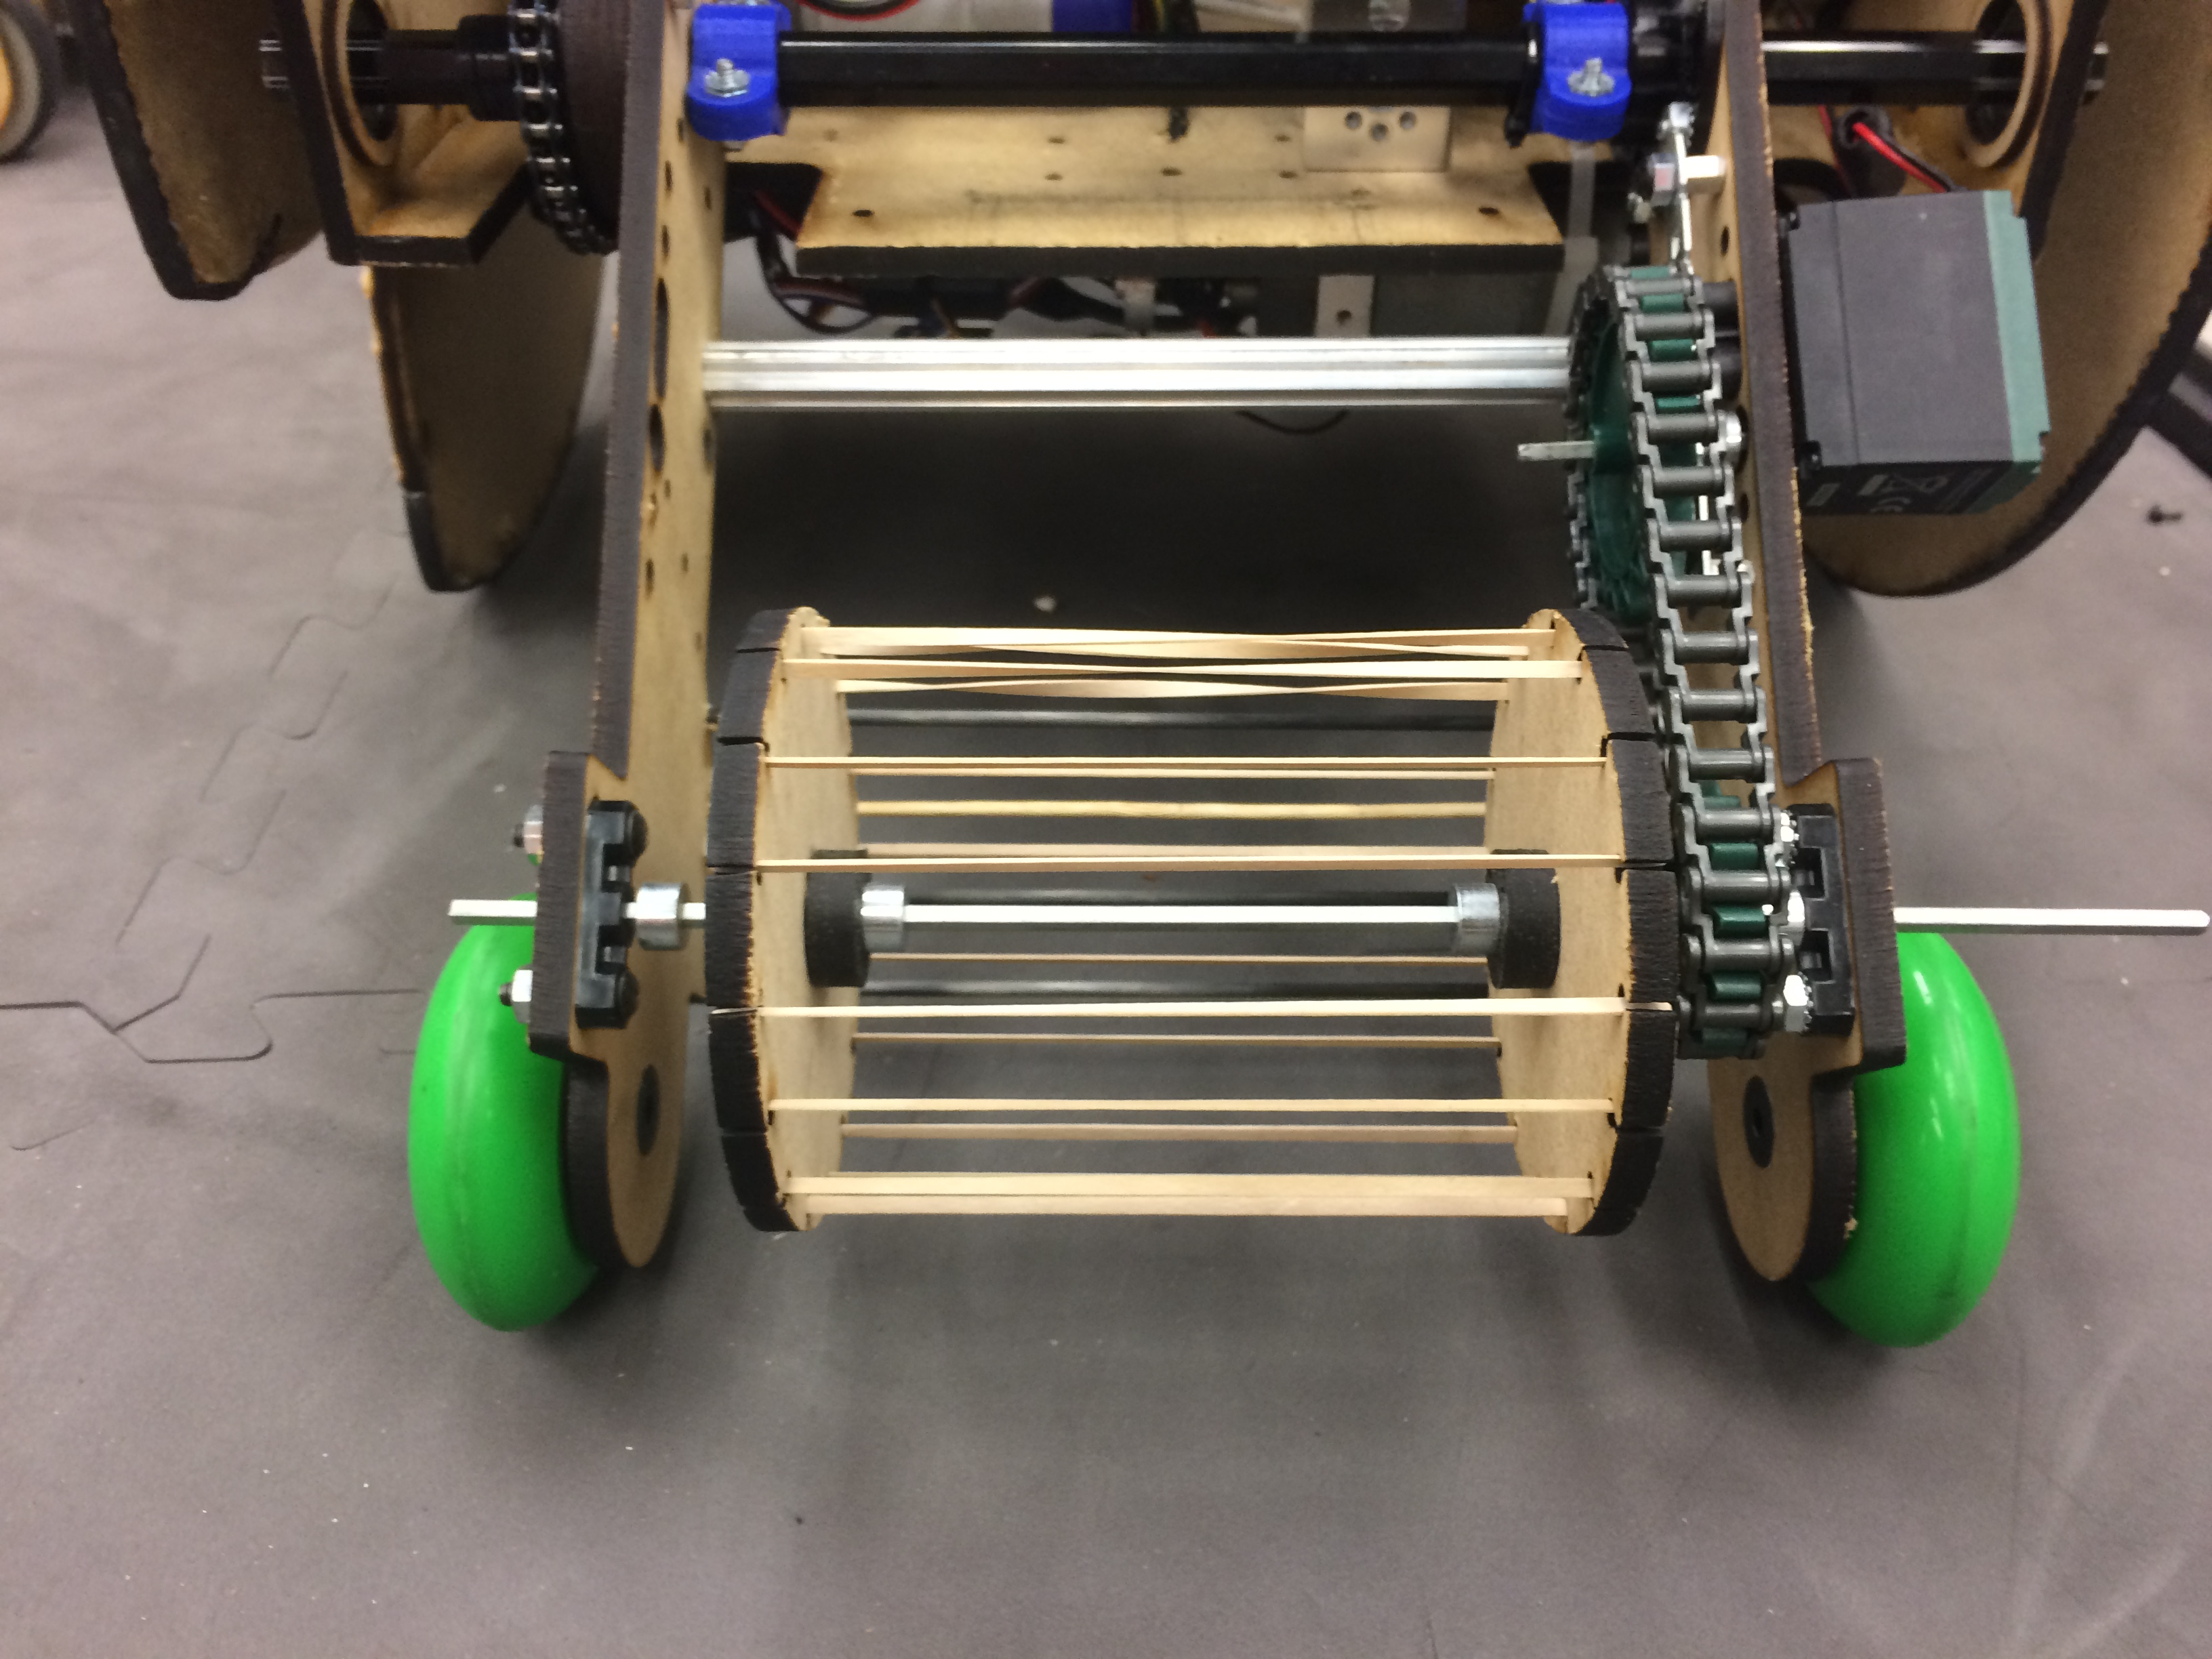
\includegraphics[width= .9\linewidth]{Design_Overview/Intake_Front.JPG}
	\caption{Final Intake, Mark V}
	\label{fig:triple_intake_IMG}
\end{minipage}%
	\hfill
\begin{minipage}{.32\textwidth}
  \centering
  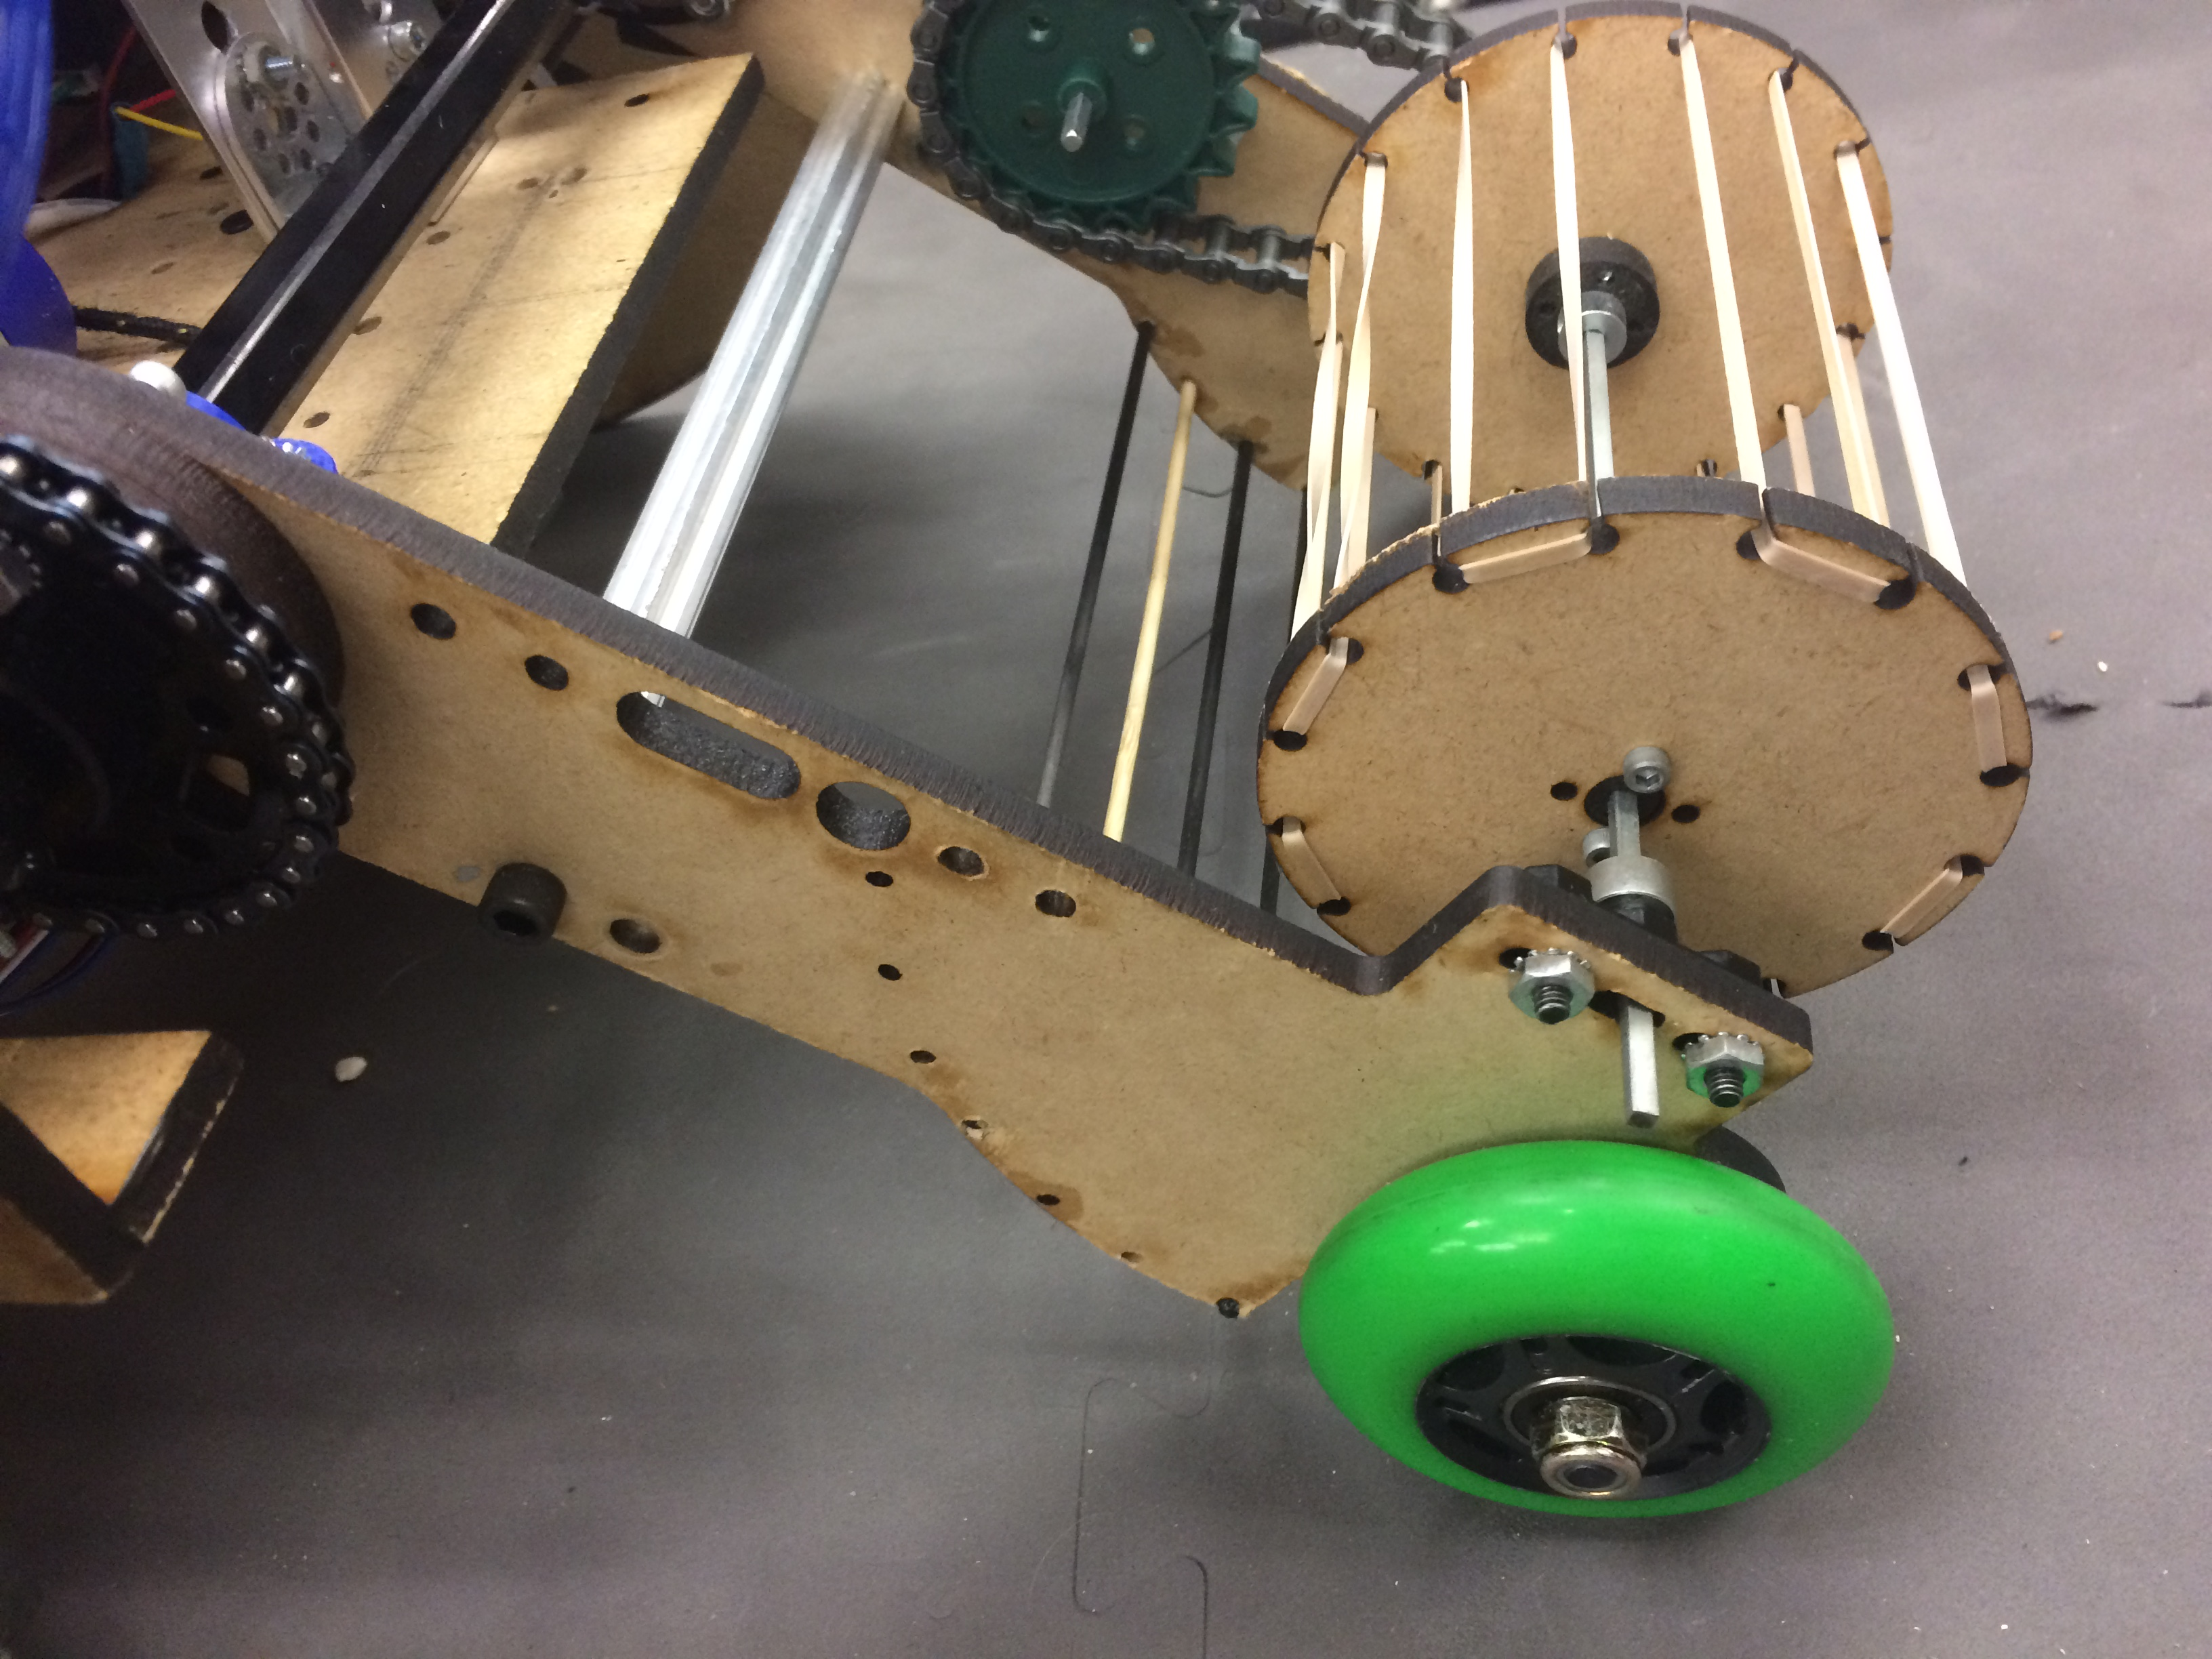
\includegraphics[width= .9\linewidth]{Design_Overview/Intake_Right.JPG}
\end{minipage}
\end{figure}